%                                                                 aa.tex
% AA vers. 9.2, LaTeX class for Astronomy & Astrophysics
% Demonstration file
%                                                       (c) EDP Sciences
%-----------------------------------------------------------------------
%
%\documentclass[referee]{aa}    % for a referee version
%\documentclass[onecolumn]{aa}  % for a paper on 1 column  
%\documentclass[longauth]{aa}   % for the long lists of affiliations
%\documentclass[letter]{aa}     % for the letters
%\documentclass[bibyear]{aa}    % if the references are not structured
                                % according to the author-year natbib style

\documentclass{aa}  

\usepackage{graphicx}
\usepackage{txfonts}
\usepackage{subcaption}         % necessary for continued figures, example in section 3
                                % and appendix
\usepackage{lscape}             % to rotate a single page table, example in appendix.
                                % For landscape tables, see the longtable examples.
\usepackage{placeins}           % useful with \FloatBarrier, to keep 
                                % onecolumn floats from drifting to the next section
\usepackage{lipsum}             % placeholder text used in template examples
% Hyperlinks and ORCID; load hyperref near the end of the preamble
\usepackage[hidelinks]{hyperref}
\usepackage{orcidlink}
% Simple flowchart support
\usepackage{tikz}
\usetikzlibrary{arrows.meta,positioning,calc,shapes.geometric}

%%%%%%%%%%%%%%%%%%%%%%%%%%%%%%%%%%%%%%%%
%\usepackage[options]{hyperref}
% To add links in your PDF file, use the package "hyperref"
% with options according to your LaTeX or PDFLaTeX drivers.
%%%%%%%%%%%%%%%%%%%%%%%%%%%%%%%%%%%%%%%%

\begin{document}

   \title{Extending PINOCCHIO to weak lensing}

   \subtitle{Particle light-cone maps}

   \author{T.~Castro\orcidlink{0000-0002-6292-3228}\inst{1,2,3,4}}

   \institute{%
   1. INAF-Osservatorio Astronomico di Trieste, Via G. B. Tiepolo 11, 34143 Trieste, Italy\and
   2. INFN, Sezione di Trieste, Via Valerio 2, 34127 Trieste TS, Italy\and
   3. IFPU, Institute for Fundamental Physics of the Universe, via Beirut 2, 34151 Trieste, Italy\and
   4. ICSC - Centro Nazionale di Ricerca in High Performance Computing, Big Data e Quantum Computing, Via Magnanelli 2, Bologna, Italy\\
   \email{tiagobscastro@gmail.com}}

   \date{\today}

% \abstract{}{}{}{}{}
% 5 {} tokens are mandatory in the A\&A class
  \abstract
  % context
  {}
  % aims
  {}
  % methods
  {}
  % results
  {}
  % conclusions
  {}

   \keywords{cosmology: large-scale structure of Universe -- gravitational lensing: weak -- methods: numerical -- catalogs}

   \maketitle

%---------------------------------------------------------------
\section{Introduction}\label{sec:intro}

%---------------------------------------------------------------
\section{Method: PLC mass-maps in PINOCCHIO}\label{sec:method}
\subsection{Overview and scope}\label{sec:method-overview}
\subsection{Algorithm orchestrator and flow}\label{sec:method-orchestrator}
This subsection provides a high-level description of the mass-maps pipeline orchestrator, introducing the end-to-end flow before detailing components. It summarizes the control logic, inputs/outputs, and error modes to guide the reader through the subsequent sections.

\paragraph{Inputs and configuration}
Simulation geometry, past light-cone (PLC) definition (observer, redshift limits, aperture), filtering options, pixelization parameters (HEALPix $N_\mathrm{side}$, RING ordering), parallel runtime settings (MPI ranks, OpenMP threads), and I/O paths.

\paragraph{Core flow}
\begin{itemize}
   \item Initialize PLC geometry, filters, and HEALPix maps; cache basis vectors and observer-centric coordinates.
   \item Iterate over time steps or particle segments along the PLC; for each segment:
   \begin{itemize}
      \item Apply fast culling (aperture, distance bounds) to skip irrelevant segments.
      \item Compute shifted positions and the sign of the PLC crossing criterion $H = \chi - r$ at segment endpoints.
      \item Detect and interpolate valid crossings; reject numerically ambiguous cases by tolerance.
      \item Convert the intersection point to sky pixel(s) and accumulate particle-level contributions.
   \end{itemize}
   \item After traversal, apply optional filters/diagnostics and finalize statistics.
   \item Write outputs: maps, tables, and FITS headers with reproducibility metadata.
\end{itemize}

\paragraph{Parallelization and I/O}
Work is distributed across MPI ranks and OpenMP threads; reductions consolidate maps and statistics; I/O is rank-gated to minimize contention. Details are expanded in Sect.~\ref{sec:method-parallel}.

   \paragraph{Contract (inputs/outputs, error modes, success)}\label{para:orchestrator-contract}
   \begin{itemize}
   \item Inputs: cosmology and simulation snapshots/segments; PLC parameters $(z_{\mathrm{min}}, z_{\mathrm{max}})$, observer position, aperture; HEALPix $N_{\mathrm{side}}$ and ordering; numerical tolerances (e.g. crossing epsilon); runtime config (MPI/OMP); output paths and flags.
      \item Outputs: particle-level HEALPix maps (and variants, if enabled); diagnostics/statistics; sheet/segment tables as needed; FITS headers with keywords for geometry, filters, seeds, and reproducibility.
      \item Error/edge modes: ambiguous crossings when $|H_\mathrm{prev}-H_\mathrm{curr}| < \varepsilon$; endpoints exactly on $H=0$; out-of-aperture segments; pixel boundary degeneracies; I/O or reduction failures (guarded with rank-gated writes and checks).
      \item Success criteria: full traversal without aborts; no NaNs/Inf in maps; counts and reductions consistent across ranks; outputs written and closed; headers populated with expected keywords.
   \end{itemize}

   \paragraph{Code references} The orchestrator delegates to well-scoped routines, including \texttt{mass\_maps\_process\_segment} (segment traversal), \texttt{mass\_maps\_crossing\_from\_shifted\_positions} (crossing detection and interpolation), \texttt{mass\_maps\_compute\_pixel\_from\_pos} (sky pixelization), and \texttt{mass\_maps\_accumulate\_entry\_pos} (map accumulation). See Sect.~\ref{sec:method-crossing} and Sect.~\ref{sec:method-pixel} for details.

\begin{figure*}[t]
\centering
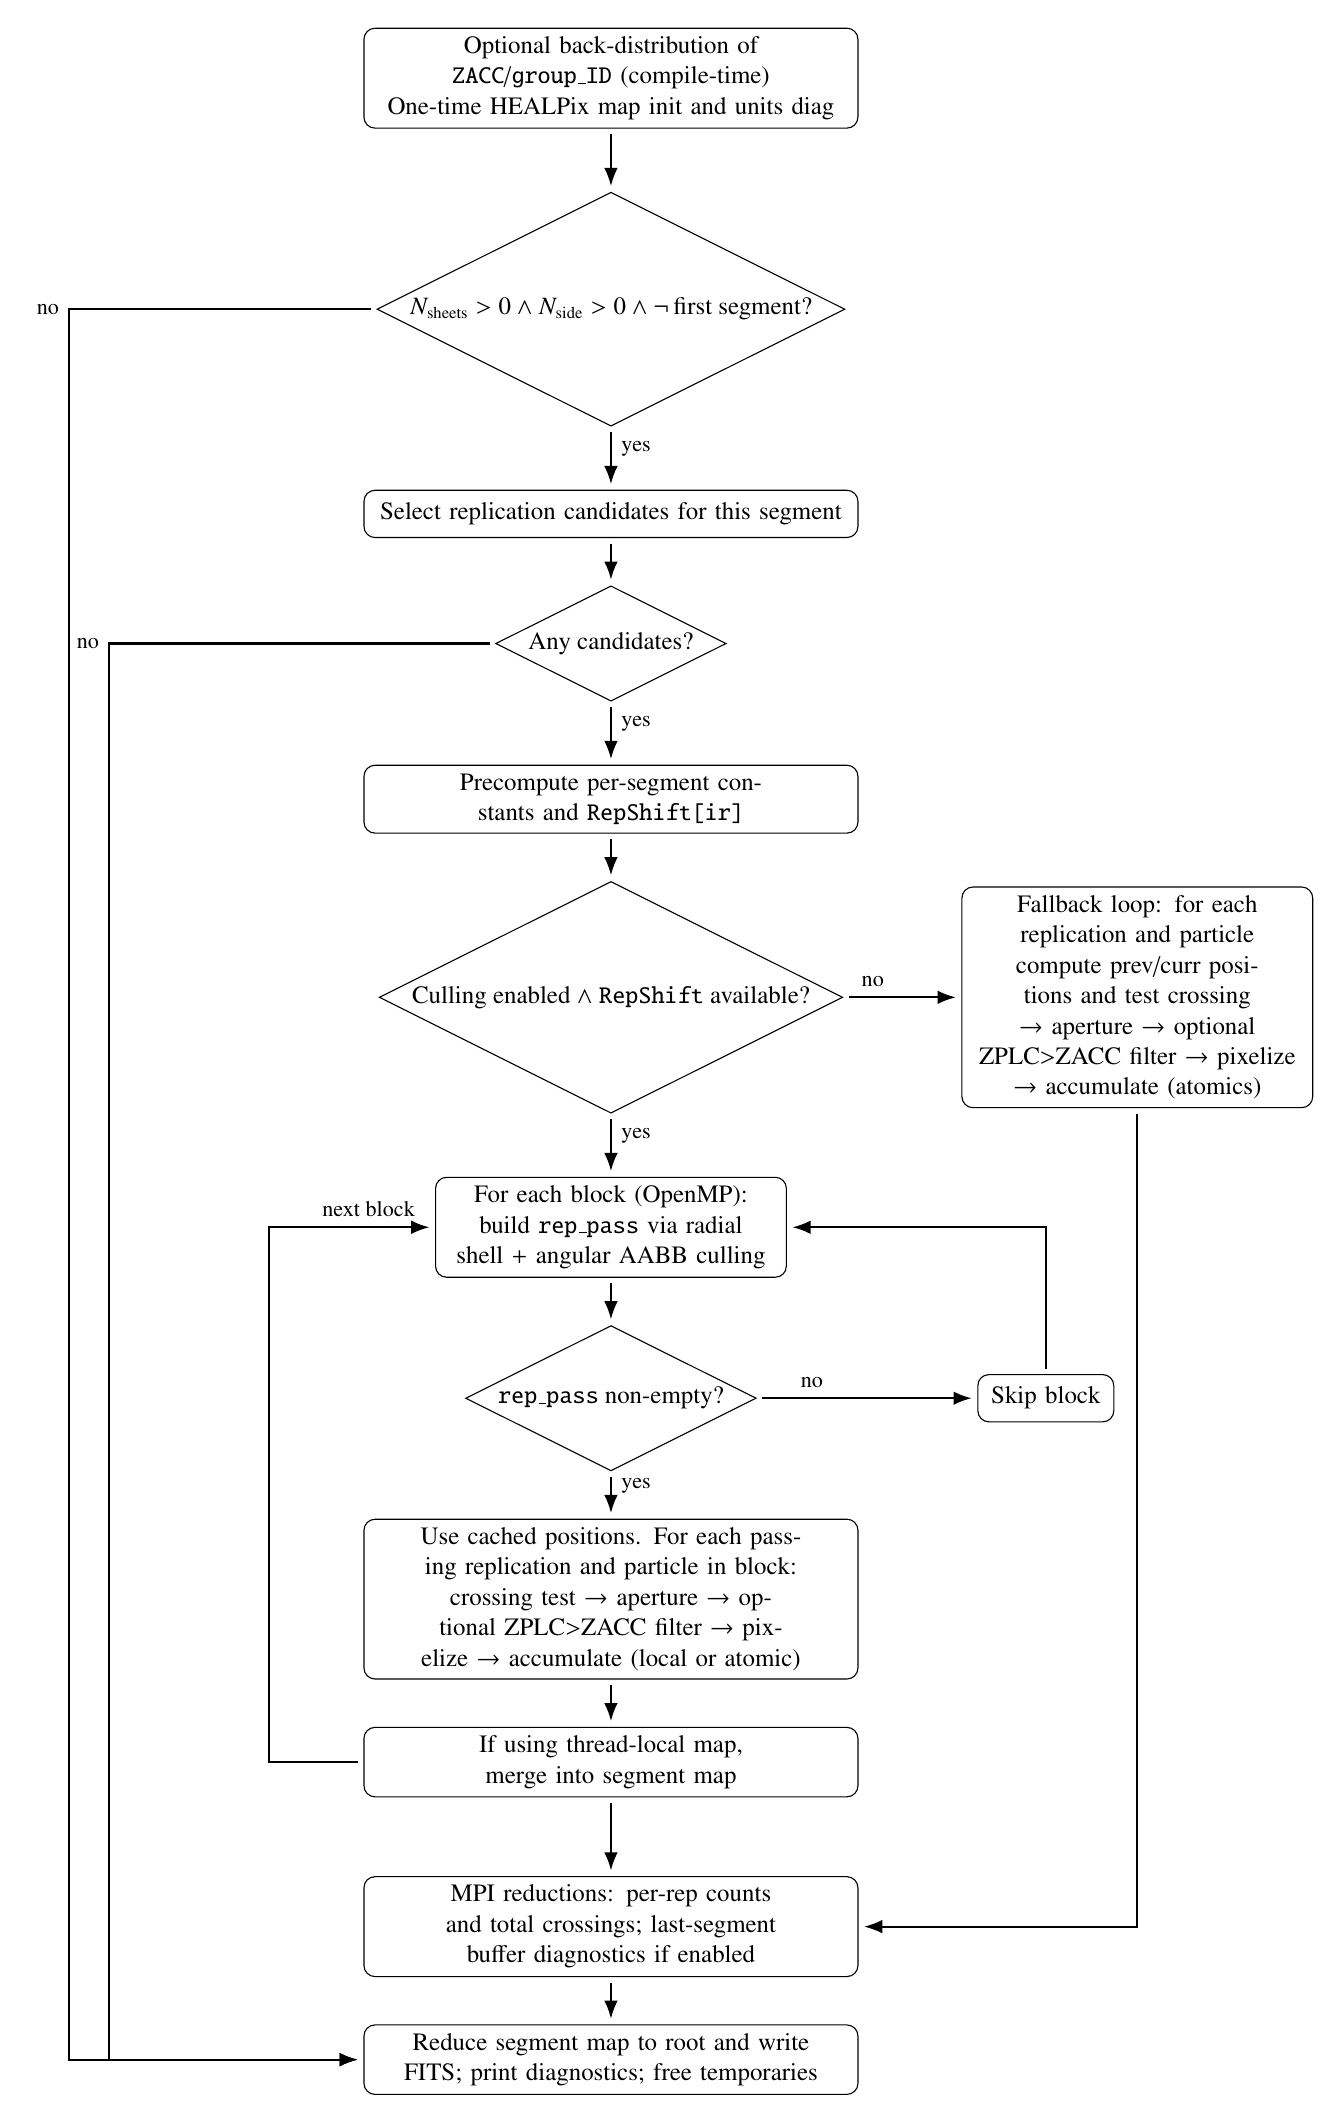
\begin{tikzpicture}[
  node distance=5mm and 10mm,
  every node/.style={font=\small},
  proc/.style={draw, rounded corners, align=center, fill=white,
               minimum height=6mm, inner sep=3pt, text width=.5\textwidth},
  decision/.style={draw, diamond, aspect=2, align=center, inner sep=1.25pt, fill=white},
  line/.style={-Latex, thick, shorten >=2pt, shorten <=2pt}
]

% ===== Spine: one segment orchestrator =====
\node[proc] (pre) {Optional back-distribution of \texttt{ZACC}/\texttt{group\_ID} (compile-time)\\One-time HEALPix map init and units diag};
\node[decision, below=8mm of pre] (gate) {$N_{\rm sheets}>0 \wedge N_{\rm side}>0 \wedge \neg\,$first segment?};
\node[proc, below=8mm of gate] (repsel) {Select replication candidates for this segment};
\node[decision, below=6mm of repsel] (repok) {Any candidates?};
\node[proc, below=8mm of repok] (prep) {Precompute per-segment constants and \texttt{RepShift[ir]}};
\node[decision, below=6mm of prep] (path) {Culling enabled $\wedge$ \texttt{RepShift} available?};

% ----- Right branch: fallback path -----
\node[proc, right=15mm of path, text width=.35\textwidth] (fallback)
  {Fallback loop: for each replication and particle\\
   compute prev/curr positions and test crossing $\rightarrow$ aperture $\rightarrow$ optional ZPLC$>$ZACC filter $\rightarrow$ pixelize $\rightarrow$ accumulate (atomics)};

% ----- Down: Culling path header -----
\node[proc, below=8mm of path, text width=.35\textwidth] (blkloop) {For each block (OpenMP): build \texttt{rep\_pass} via radial shell + angular AABB culling};
\node[decision, below=6mm of blkloop] (passok) {\texttt{rep\_pass} non-empty?};
\node[proc, right=28mm of passok, text width=.125\textwidth] (skipblk) {Skip block};
\node[proc, below=6mm of passok] (inner)
  {Use cached positions. For each passing replication and particle in block:\\
   crossing test $\rightarrow$ aperture $\rightarrow$ optional ZPLC$>$ZACC filter $\rightarrow$ pixelize $\rightarrow$ accumulate (local or atomic)};
\node[proc, below=6mm of inner] (merge) {If using thread-local map, merge into segment map};

% ----- Tail: reductions and outputs -----
\node[proc, below=10mm of merge] (reduce)
  {MPI reductions: per-rep counts and total crossings; last-segment buffer diagnostics if enabled};
\node[proc, below=6mm of reduce] (write)
  {Reduce segment map to root and write FITS; print diagnostics; free temporaries};

% ===== Edges: spine and branches =====
\draw[line] (pre) -- (gate);
\draw[line] (gate) -- node[right,pos=.35]{\footnotesize yes} (repsel);
\draw[line] (gate.west) -- ++(-39mm,0) node[left]{\footnotesize no} |- (write.west); % early exit to end

\draw[line] (repsel) -- (repok);
\draw[line] (repok) -- node[right,pos=.35]{\footnotesize yes} (prep);
\draw[line] (repok.west) -- ++(-49mm,0) node[left]{\footnotesize no} |- (write.west); % no reps → return

\draw[line] (prep) -- (path);
\draw[line] (path.east) -- node[above, near start]{\footnotesize no} (fallback.west);
\draw[line] (path) -- node[right,pos=.35]{\footnotesize yes} (blkloop);

\draw[line] (blkloop) -- (passok);
\draw[line] (passok.east) -- node[above, near start]{\footnotesize no} (skipblk.west);
\draw[line] (skipblk.north) |- (blkloop.east);

\draw[line] (passok) -- node[right,pos=.3]{\footnotesize yes} (inner);
\draw[line] (inner) -- (merge);

% External left rail for block iteration
\path let \p1=(pre.west), \p2=(merge.west), \p3=(blkloop.west) in
      coordinate (railLow)  at (\x1-12mm,\y2)
      coordinate (railHigh) at (\x1-12mm,\y3);
\draw[line] (merge.west) -- (railLow) -- (railHigh) --  node[above,pos=.6]{\footnotesize next block} (blkloop.west);

% Join both paths to tail
\draw[line] (fallback.south) |- (reduce.east);
\draw[line] (merge) -- (reduce);
\draw[line] (reduce) -- (write);

% Caption reminder:
\end{tikzpicture}
\caption{Per-segment orchestrator in \texttt{mass\_maps\_process\_segment}: initialization, replication selection, culling or fallback traversal, crossing, aperture filter, pixelization, accumulation, and final MPI reduction and FITS output.}
\label{fig:orchestrator-flow}
\end{figure*}


\subsection{Geometry and PLC definition}\label{sec:method-geometry}
\subsection{Crossing detection and interpolation}\label{sec:method-crossing}
\subsection{Pixelization and map accumulation}\label{sec:method-pixel}
\subsection{Filtering, diagnostics, and outputs}\label{sec:method-filter}
\subsection{Parallelization and performance}\label{sec:method-parallel}

%---------------------------------------------------------------
\section{Validation}\label{sec:validation}
\subsection{Numerical checks and convergence}\label{sec:validation-conv}
\subsection{Comparison to external references}\label{sec:validation-compare}
\subsection{Performance benchmarks}\label{sec:validation-perf}

%---------------------------------------------------------------
\section{Results}\label{sec:results}
\subsection{Example light-cone maps}\label{sec:results-examples}
\subsection{Science use cases}\label{sec:results-usecases}

%---------------------------------------------------------------
\section{Discussion}\label{sec:discussion}

%---------------------------------------------------------------
\section{Conclusions}\label{sec:conclusions}

%---------------------------------------------------------------
\section{Data and software availability}\label{sec:data}

%---------------------------------------------------------------
\begin{acknowledgements}
% Acknowledgements
\end{acknowledgements}

\bibliographystyle{aa}
\bibliography{paper}

\begin{appendix}
\section{FITS header keywords}\label{app:fits}
\section{Run-time parameters and defaults}\label{app:params}
\end{appendix}
\end{document}